%===============================================================================
% Template Name:      SUnORE Starter Presentation template
% Template URI:       http://sunore.co.za/sunore-presentation/
% Description:        Starter Presentation template for SUnORE 
%                     Department of Industrial Engineering, 
%                     Stellenbosch University
% Version:            1.1.0
% Author:             Johan Janse van Rensburg
% Author URI:         http://johanjvrens.co.za/
% License:            MIT License
% License URI:        http://opensource.org/licenses/MIT
%===============================================================================
\documentclass[serif,11pt]{beamer}

%=================================================
% theme and color
%=================================================
\usetheme{Warsaw} %Themes http://www.hartwork.org/beamer-theme-matrix/
\definecolor{colorA}{RGB}{96, 34, 59}
\definecolor{colorB}{RGB}{140, 151, 154}
%\definecolor{secinhead}{RGB}{249,196,95}
%\definecolor{titlebg}{RGB}{51,51,51}
\setbeamercolor{structure}{fg=colorA,bg=colorB}
%\setbeamercolor{secsubsec}{fg=secinhead,bg=black}
%\setbeamercolor{frametitle}{fg=secinhead,bg=titlebg}

%=================================================
% packages and new commands
%=================================================
\usepackage[ruled, linesnumbered, vlined]{algorithm2e}
\usepackage{epsfig, subfigure, amssymb, multirow, algorithmic, amsmath}
\newcommand*{\superscript}[1]{\ensuremath{^{\rm #1}}}
\newcommand*{\subscript}[1]{\ensuremath{_{\rm #1}}}

%=================================================
% thesis details (preamble)
%=================================================
\title[{\sc The short title of your thesis } \hspace{0.8cm} \insertframenumber/\inserttotalframenumber]{{\sc The title of your thesis or dissertation should be typed here }}
\author[Presentation to some students --- {\sc Feb 10\superscript{th}, 2015}]{{Student name}}
\date{10 Feb 2015}
\institute{Operations Research Group \\ Department of Industrial Engineering \\ Stellenbosch University, South Africa}

%=================================================
% start presentation
%=================================================
\begin{document}

%========================
% title page
%========================
\begin{frame}
  \begin{center}
    \vspace{0.1cm}
    
\includegraphics[scale=0.25]{USlogo.pdf}
  \end{center}
  \titlepage
\end{frame}

%========================
% your slides:
%========================
\begin{frame}\frametitle{Overview}
\begin{itemize}
\pause \item The trivial Set Cover algorithm has running time of ${\cal O}(2^n)$.
\pause \item bla, bla, bla\ldots
\end{itemize}

\end{frame}

%========================
% example slides:
%========================
%\section{Lists}
% --------------------------------------------------- Slide --
%\subsection{Itemize}
\label{itemize}
\begin{frame}\frametitle{Lists - Itemize}
  \begin{itemize}
    \item Point A
    \item Point B
    \begin{itemize}
      \item part 1
      \item part 2
    \end{itemize}
    \item Point C
    \item Point D
  \end{itemize}
\end{frame}

% --------------------------------------------------- Slide --
%\subsection{Pause}
\label{pause}
\begin{frame}\frametitle{Lists - Itemize with Pause}
  \begin{itemize}
    \pause \item Point A
    \pause \item Point B
    \begin{itemize}
      \pause \item part 1
      \pause \item part 2
    \end{itemize}
    \pause \item Point C
    \pause \item Point D
  \end{itemize}
\end{frame}

% --------------------------------------------------- Slide --
%\subsection{Enumerate}
\label{enumerate}
\begin{frame}\frametitle{Lists - Enumerate}
  \begin{enumerate}
    \item Point A
    \item Point B
    \begin{enumerate}
      \item part 1
      \item part 2
    \end{enumerate}
    \item Point C
    \item Point D
  \end{enumerate}
\end{frame}

% --------------------------------------------------- Slide --
%\subsection{Enumerate (Roman Numerals)}
\label{enumerateRomanNumerals}
\begin{frame}\frametitle{Lists - Enumerate (Roman Numerals)}
  \begin{enumerate} [(I)]
	\item Point A
	\item Point B
	\begin{enumerate} [(i)]
	  \item part 1
      \item part 2
	\end{enumerate}
	\item Point C
	\item Point D
  \end{enumerate}
\end{frame}
\begin{frame}\frametitle{Columns}

\begin{columns}
\column{0.5\textwidth}
Lorem ipsum dolor sit amet, consectetur adipisicing elit, sed do eiusmod tempor incididunt ut labore et dolore magna aliqua.
\column{0.5\textwidth}
Lorem ipsum dolor sit amet, consectetur adipisicing elit, sed do eiusmod tempor incididunt ut labore et dolore magna aliqua.
\end{columns}

\end{frame}
\begin{frame}\frametitle{Domination on a Chessboard}
\begin{figure}[htb]
\centering
 \begin{tabular}{cc}\pause{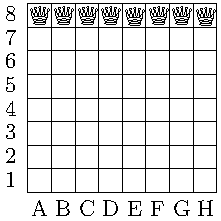
\includegraphics[scale=1]{examples/DomChess8.pdf}}&
       \pause{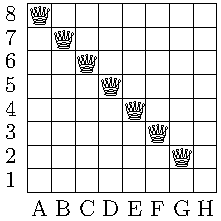
\includegraphics[scale=1]{examples/DomChess7.pdf}}\\
       \pause{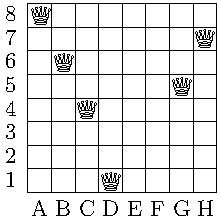
\includegraphics[scale=1]{examples/DomChess6.pdf}}&
      \pause{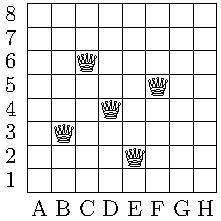
\includegraphics[scale=1]{examples/Chess1.pdf}}
      \end{tabular}
\end{figure}
\end{frame}
\begin{frame}\frametitle{Description Environment}

\begin{description}
\item[API] Application Programming Interface
\item[LAN] Local Area Network
\item[ASCII] American Standard Code for Information Interchange
\end{description}

\end{frame}
\begin{frame}\frametitle{Tables}

\begin{table}
\begin{tabular}{l | c | c | c | c }
Competitor Name & Swim & Cycle & Run & Total \\
\hline \hline
John T & 13:04 & 24:15 & 18:34 & 55:53 \\ 
Norman P & 8:00 & 22:45 & 23:02 & 53:47\\
Alex K & 14:00 & 28:00 & n/a & n/a\\
Sarah H & 9:22 & 21:10 & 24:03 & 54:35 
\end{tabular}
\caption{Triathlon results}
\end{table}

\end{frame}
\begin{frame}\frametitle{Blocks}

\begin{block}{Block Title}
Lorem ipsum dolor sit amet, consectetur adipisicing elit, sed do eiusmod tempor incididunt ut labore et dolore magna aliqua.
\end{block}

\begin{alertblock}{Block Title}
Lorem ipsum dolor sit amet, consectetur adipisicing elit, sed do eiusmod tempor incididunt ut labore et dolore magna aliqua.
\end{alertblock}

\end{frame}
%\section{Definition}
% --------------------------------------------------- Slide --
%\subsection{Definition}
\label{definition}
\begin{frame}\frametitle{Definition}
  Then there’s the definition environment which produces a standard ColorA color block but with the title already specified as ‘definition’.
  \begin{semiverbatim}
    \\begin\{definition\}\newline
    A prime number is a number that...\newline
    \\end\{definition\}
  \end{semiverbatim}
  \begin{definition}
    A prime number is a number that...
  \end{definition}
\end{frame}
\begin{frame}\frametitle{Example}

\begin{example}
Lorem ipsum dolor sit amet, consectetur adipisicing elit, sed do eiusmod tempor incididunt ut labore et dolore magna aliqua.
\end{example} 

\end{frame}
%\section{Theorem}
% --------------------------------------------------- Slide --
%\subsection{Theorem Code}
\label{theoremCode}
\begin{frame}\frametitle{Theorem}
  There is also a group of blocks that are especially useful for presenting mathematics. For example the ‘theorem’ environment, the ‘corollary’ environment and the ‘proof’ environment.
  \begin{semiverbatim}
    \\begin\{theorem\}[Pythagoras] \newline
      $ a^2 + b^2 = c^2$ \newline
    \\end\{theorem\} \newline
    \\begin\{corollary\} \newline
      $ x + y = y + x  $ \newline
    \\end\{corollary\} \newline
    \\begin\{proof\} \newline
      $\omega +\phi = \epsilon $ \newline
    \\end\{proof\}
  \end{semiverbatim}
\end{frame}

% --------------------------------------------------- Slide --
%\subsection{Theorem Blocks}
\label{theoremBlocks}
\begin{frame}\frametitle{Theorem Blocks}
  \begin{theorem}[Pythagoras] 
    $ a^2 + b^2 = c^2$
  \end{theorem}
  \begin{corollary}
    $ x + y = y + x  $
  \end{corollary}
  \begin{proof}
    $\omega +\phi = \epsilon $
  \end{proof}
\end{frame}
%\section{Hyperlinks}
% --------------------------------------------------- Slide --
%\subsection{Hyperlinks Code}
\label{hyperlinks}
\begin{frame}\frametitle{Hyperlink}
Before we can create any hyperlinks we need to tag the frames we want to link to using the \label command.
 
\hyperlink{contents}{click here}
\hyperlink{section1}{\beamerbutton{section 1 page}}
\hyperlink{columns}{\beamergotobutton{columns page}}
\hyperlink{pictures}{\beamerskipbutton{pictures page}}
\hyperlink{pictures}{\beamerreturnbutton{pictures page}}

\end{frame}
\SetKwInOut{Input}{Input}\SetKwInOut{Output}{Output}
\begin{frame}\frametitle{A trivial Set Cover algorithm}
\begin{algorithm}[H]\footnotesize
        \Input{A set cover instance $({\cal S,U})$ and a variable ${\cal S}_{\rm dom}$.}
        \Output{A minimum set cover of $({\cal S,U})$.}
\If{${\cal S}=\emptyset$}{
\Return $\emptyset$\;
}
Let $S \in {\cal{S}}$ be a set of maximum cardinality\;
${\cal{C}}_1 = \{S\}\cup {\tt MSC}(\{S'\backslash S \mid S' \in{\cal S}\backslash \{S\}\}, {\cal U}\backslash S )$\;
${\cal{C}}_2 = {\tt MSC}({\cal S}\backslash \{S\},{\cal U})$\;
${\cal S}_{\rm dom} \leftarrow \emptyset$\;
\If{${\cal U} \subseteq {\cal C}_1$}{
${\cal S}_{\rm dom} \leftarrow {\cal C}_1$\;
\If{${\cal U} \subseteq {\cal C}_2$}{
\If{$|{\cal C}_2| < |{\cal C}_1|$}{
${\cal S}_{\rm dom} \leftarrow {\cal C}_2$\;
}
}
}
\Return ${\cal S}_{\rm dom}$\;
\caption{{\tt MSC}$({\cal S,U})$}
\end{algorithm}
\end{frame}

%========================
% bibliography
%========================
%%%%%%%%%%%%%%%%%%
%
% bibliography
%
%%%%%%%%%%%%%%%%%%

\begin{frame} \frametitle{References}
\begin{thebibliography}{xx}\footnotesize

\bibitem{FominFVGrandoniFKratschD2009} {\sc Fomin FV, Grandoni F \& Kratsch D}, 2009, {\em A note on the complexity of minimum dominating set }, Journal of Discrete Algorithms, {\bf{4(2)}}, pp.\ 209--214.

\bibitem{critical} {\sc Grobler PJP \& Mynhardt CM}, 2009, {\em Secure domination critical graphs}, Discrete Mathematics, {\bf 309}, pp.~5820--5827.

\bibitem{VRB}{{\sc Van Rooij JMM \& Bodlaender HL}, 2011, {\em Exact algorithms for dominating set}, Discrete Applied Mathematics, {\bf 159}, pp.\ 2147--2164.}

\end{thebibliography}
\end{frame}

%=================================================
% end presentation
%=================================================
\end{document}